\chapter{Latex Beispiel}
\thispagestyle{fancy}
\label{LatexBeispiel}
Über das chapter Steuerzeichen werden Überschriften generiert.\\
Über das label Steuerzeichen können Referenzmarken geschaffen werden die über \mbox{(siehe Kap. \ref{LatexBeispiel}  S. \pageref{LatexBeispiel})} referenziert werden können.
Dazu muss jedoch das Dokument zwei Mal berechnet werden.
\section{Unter einem Chapter kommt eine Section}
Eine Section wird numeriert und taucht im Inhaltsverzeichnis auf.
\subsection{Unter einer Section eine Subsection}
Eine SubSection wird numeriert und taucht im Inhaltsverzeichnis auf.
\subsubsection{Unter einer Subsection eine SubSubSection}
Eine SubSubSection wird numeriert und taucht in diesem Falle nicht im Inhaltsverzeichnis auf.
\paragraph{Ein Paragraph}$\;$\\
Ein Paragraph erhält keine Nummerierung, dafür eine fette Überschrift und wird nicht im Inhaltsverzeichnis aufgezählt.
\\ %Leerzeile
Fußnote\footnote{\mbox{Innenwiderstand $20m\Omega$ $\rightarrow$ $\frac{1,35V-0,85V}{20m\Omega}=25A$ Ladestrom}} mit grenzeneinhaltender Mathematik.
Einfache Elemente kann man auch so: $V_{high}$ einbinden.
oder als numerierte Equation
\begin{equation} \label{eq:Tiefpass24}
|A|=\sqrt{\frac{(1-\omega^{2}R_{1}C_{1}R_{2}C_{2})^{2}+(\omega(R_{1}C_{1}+R_{2}C_{2}))^{2}}{\left( (1-\omega^{2}R_{1}C_{1}R_{2}C_{2})^{2}+(\omega(R_{1}C_{1}+R_{2}C_{2}))^{2}\right)^{2}}}
\end{equation}

Zitiere Eric C. Darcy\cite{Darcy} aus der Bibliothek.

\begin{figure}[ht!]
\centering
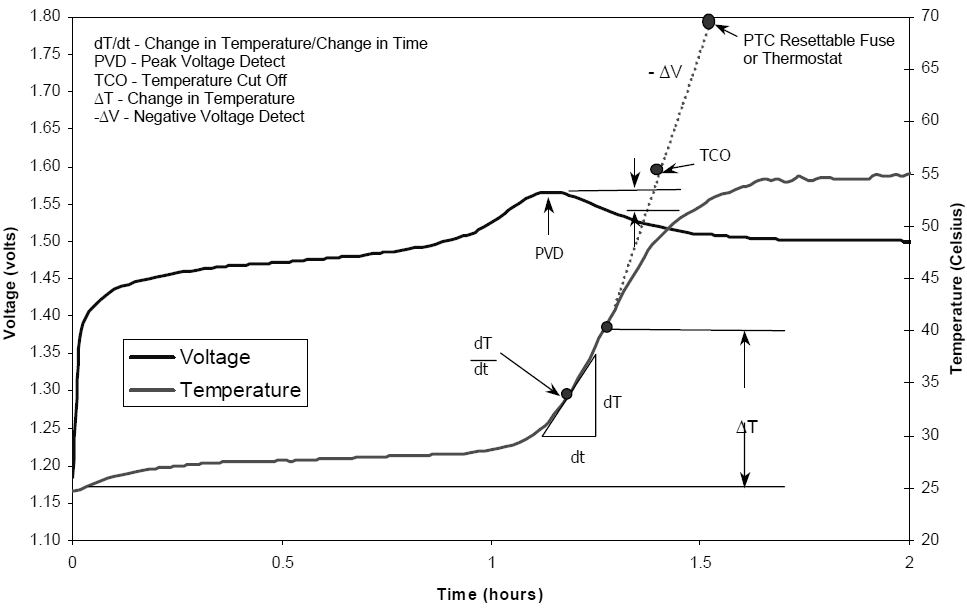
\includegraphics[angle=0,width=14cm]{LatexBeispiel/Bilder/Ladeschlussbw.png}
\caption{Ladeschlusserkennungen, Harding Battery Handbook\cite{Harding}}
\label{Ladeschluss}
\end{figure}

\newpage
So kann Code eingefügt werden.
\begin{lstlisting}[frame=single,breaklines=true,basicstyle=\tiny,language=C,label={PWMStart},caption={Kommentierter Start der PWM}]
/*! \brief Starts the PWM
 * 
 * To make sure that the PWM behaves correctly after a Compare Bit Change the PWM is started and reset with a software trigger.
 */
static void vStartPwm( void )
{
	tc_start( &AVR32_TC0, PWM_CHANNEL );
	tc_software_trigger( &AVR32_TC0, PWM_CHANNEL );
}
\end{lstlisting}
